\documentclass[12pt]{article}
% Préambule commun à tous les documents extraits de « La Revue CAPES »
\usepackage[T1]{fontenc}
\usepackage[utf8]{inputenc}
\usepackage{lmodern}
\usepackage{amsmath,amssymb,amsthm,amsfonts,mathrsfs}
\usepackage{setspace}
\usepackage{listings}
\usepackage{pgfplots}
\pgfplotsset{compat=1.18}
\usepackage{longtable}
\usepackage{adjustbox}
\usepackage{lettrine}
\usepackage{tkz-tab}
\usepackage{changepage}
\usepackage{pdflscape}
\usepackage{graphicx}
\usepackage{tikz}
\usepackage{xcolor}
\usepackage[a4paper,top=2cm,bottom=2.5cm,left=2.5cm,right=2cm]{geometry}
\usepackage{fancyhdr}
\usepackage{draftwatermark}
\SetWatermarkText{La RevueCapes}
\SetWatermarkLightness{0.9}
\SetWatermarkScale{2}
\usepackage{hyperref}
\hypersetup{colorlinks=true,linkcolor=blue!50!black,urlcolor=blue!50!black}

\definecolor{revue}{RGB}{20,60,120}

\pagestyle{fancy}
\fancyhf{}
\renewcommand{\headrulewidth}{0.4pt}
\setlength{\headheight}{15pt}

% \entete{Matière}{Titre}{Type de document}
\newcommand{\entete}[3]{%
  \fancyhead[L]{\small\textsc{La Revue CAPES} -- #1}%
  \fancyhead[R]{\small #2}%
  \fancyfoot[C]{\thepage}%
  \thispagestyle{plain}%
  \begin{center}
    {\color{revue}\rule{\textwidth}{1.2pt}}\\[4pt]
    {\small\textsc{Concours directs CAP-CEG / CAPES -- Burkina Faso}}\\[6pt]
    {\LARGE\bfseries\color{revue} #2}\\[6pt]
    {\large\itshape #1 -- #3}\\[2pt]
    {\color{revue}\rule{\textwidth}{1.2pt}}
  \end{center}
  \vspace{0.5cm}%
}

% Encadré pour les remarques ajoutées dans les corrigés
\newcommand{\remarque}[1]{\par\medskip\noindent\fcolorbox{revue}{revue!6}{\parbox{\dimexpr\linewidth-2\fboxsep-2\fboxrule}{\textbf{\color{revue}Remarque.} #1}}\par\medskip}


\begin{document}
\entete{Mathématiques}{Corrigé détaillé du sujet type n°13}{Correction}
\begin{spacing}{1.5}

\textbf{Exercice 1}

\textbf{Partie 1}

Soit $A$ un réel non nul. 

Montrer que, pour tout $n$ entier naturel non nul, on peut déterminer une suite unique de $n+1$ 
nombres réels $(t_0, t_1, ….t_{n-1},t_n)$ vérifiant les trois conditions suivantes : 

(i)    $t_0 = 0, t_n = A$ 

(ii)   $t_0 < t_1 < ….t_{n-1} < t_n$

(iii)  $\forall k\in \lbrace 0, ...., n-1\rbrace, t_{k+1}-t_{k}= A/n$

En procédant par récurrence avec la dernière condition, on a :

$t_{1}-t_{0}= A/n\Rightarrow t_1=A/n$ puisque $t_0=0$

$t_2-t_1=A/n \Rightarrow t_2=2A/n$

$t_3-t_2=A/n \Rightarrow t_3=3A/n$

$\vdots$					$\vdots$

$t_k=kA/n$ pour $k$ allant de 0 à $n$.

\medskip\textbf{Partie 2}

Posons $F(x)=\int_0^xf(t).dt$  qui existe d'après les hypothèses sur $f$ ; en outre la dérivée 
$F'(x) =f(x) > 0$ donc $F$ est strictement croissante sur $[0,1]$, et $F$ est donc inversible. 

Posons $t_k = F(x_k)$, et $A = \int_0^1f(t).dt$

On cherche une suite de $n+1$ nombres entre 0 et 1 vérifiant les 3 conditions de la partie 1 :  

(i)    $t_0 = 0, t_n = A$ 
(ii)   $t_0 < t_1 < ….t_{n-1} < t_n$
(iii)  $\forall k\in \lbrace 0, ...., n-1\rbrace, t_{k+1}-t_{k}= A/n$

Donc $t_k = kA/n$, pour $k$ allant de 0 à $n$. 

D'où $x_k = F^{-1}(kA/n)$, pour $k$ allant de 0 à $n$. 

En outre, puisque $F$ et donc $F-1$ sont strictement croissantes, les $x_k$ sont rangés en ordre croissant $x_0 < x_1 < ….. x_{n-1} < x_n$   

 2) $U(n) =\frac{1}{n}\sum_{k=0}^nf(x_k)= \frac{1}{n}\sum_{k=0}^nf(F^{-1}(kA/n))$ qui converge vers :
 
 \[
 A^{-1}\int_0^Af(F^{-1}(t))dt=\frac{B}{A}\] ou \[B=\int_0^Af(F^{-1}(t))dt\]
 
 Faisons le changement de variable $u=F^{-1}(t)$, ou $t=F(u)$, $dt=f(u)du$
 
 \[
 B=\int_0^1f(u)f(u)du=\int_0^1f^2(u)du\]
 
 On en déduit que \[L=\frac{\int_0^1f^2(u)du}{\int_0^1f(u)du}\]

3) Un calcul simple donne $A=e-1$
 
 De même, $x_k=ln(k(e-1)/n)$
 
 $B =(e^2-1)/2$ et donc $L=(e+1)/2$
 
 \medskip\textbf{Exercice 2}
 
 $g(x)=\frac{1}{lnx}$
 
 1) Il est évident que $g$ est définie sur $\mathbb{R}_+^{\ast}$ sauf pour $x = 1$. 

\underline{Dérivée :} $g'(x) =-\frac{1}{xln^2x}< 0 \forall x \in \mathbb{R}_+^{\ast}\setminus\{1\}$. 

Donc $g$ est décroissante. 

De même,$ g''(x) = (2 + lnx)/x^2ln^3x$ qui s'annule en $x = e^{-2} $

Donc $g$ admet un point d'inflexion en $x = e^{-2}$ et $g(e^{-2}) =-\frac{1}{2}$. 

\underline{Limites :}
 
Quand $x\rightarrow 0^+$, $g$ tend vers 0. 

Quand $x\rightarrow 1^-$, $g$ tend vers $-\infty$
 
Quand $x\rightarrow 1^+$, $g$ tend vers $+\infty$
 
Quand $x\rightarrow +\infty$, $g$ tend vers 0.
 
\underline{Asymptotes :} $x = 1, x = 0$ (vers $+\infty$)

\underline{Tableau de variation} 

\begin{center}
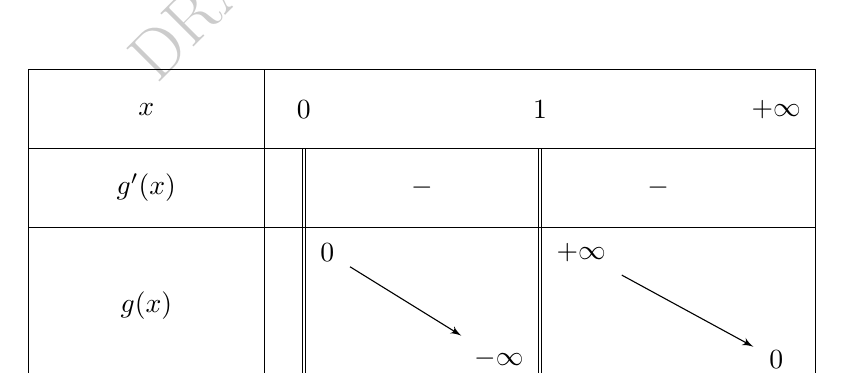
\begin{tikzpicture} 
\tkzTabInit[lgt=3, espcl=3]{$x$ /1, $g'(x)$ /1, $g(x)$ /2}{$0$, $1$, $+\infty$} 
\tkzTabLine{d, -, d, -,} 
\tkzTabVar{D+/$0$, -D+/ $-\infty$/$+\infty$ , -/$0$}
\end{tikzpicture} 
\end{center}


\underline{Graphe}

\quad

2) On considère l'ensemble $D = ]0,1/2[\cup]1,+\infty[$.

On définit l'intégrale $J(x)$ par : 
$J(x) =\int_{x}^{2x}g(t)dt$

Montrons que $J(x)$ existe pour tout $x\in D$.

 L'intégrale n'existe que si 1 n'est pas dans l'intervalle $(x, 2x)$, soit $1 < x$ ou $1 > 2x$, 
donc $x <1/2$ ou$ x > 1$, ce qui correspond à $D$. 

Avec la notation introduite en Q1), $J(x) = G(2x)-G(x)$. 

3) Soit l'ensemble $D^+ = [0,1/2[\cup ]1,+\infty[ = D \cup \lbrace 0\rbrace$

On définit l'application $f : D^+\longrightarrow \mathbb{R}$ par : 

$\forall x \in D,f(x) = J(x)$

$f(0)=0$

Montrer que $f$ est dérivable sur $D$, et calculer sa dérivée $f^{\prime}$.

Étudier le signe de $f^{\prime}$ et en déduire le sens des variations de $f$ 

Sur $D, J(x)= G(2x)-G(x)$, et donc, puisque $G'= g$, on a :$f'(x)$ existe et vaut : 
\[
f'(x) = 2g(2x)-g(x) = ln(x/2) /[(Lnx)(Ln2x)]\]

$\longrightarrow$ Pour pour $x < 1/2$, $f'(x)$ est $<0$, donc $f$ est décroissante. 

$\longrightarrow$ Pour $x > 1$, $f'(x)$ est $> 0$ si $x /2 > 1$, donc $x > 2$ ; de même, $f'(x) < 0$ si $x < 2$, et on a 
$f'(x) = 0$ si $x = 2$. 

On remarque aussi que la limite de $f'$ quand $x$ tend vers 0 est égale à 0. 
 
4) D'après les accroissements finis appliqués à $f$, $f = (2x-x)g(c), x \leqslant c \leqslant 2x$. 

Comme la fonction $g$ est décroissante (question 1), $g(x)\geqslant g(c)\geqslant g(2x)$, donc : 

\[x/\ln(2x)\leqslant f(x)\leqslant x/\ln x\]

et 

\[1/\ln(2x)\leqslant f(x)\leqslant 1/\ln x\]
 
On en déduit quand $x$ tend vers 0 : 

a) $f(x)$ tend vers 0 

b) $f(x) / x$ tend vers 0 

Donc on peut prolonger $f$ par continuité en 0. 

De même, la limite de $(f(x)-f (0))/(x-0) =f(x) /x$ est égale à 0, qui est aussi la limite 
de $f'$ en 0 (remarque de la question 3), donc $f$ est dérivable en 0. 

5) Toujours en utilisant la double inégalité de la question 4, on a : 
Quand $x$ tend vers $+\infty$ : 

a) $f(x)$ tend vers $+\infty$ 

b) $f(x) / x$ tend vers 0 

6) En étudiant brièvement $h(u)$ sur $]0, 1]$, on voit que $h$ est croissante de $-\infty$ à $1-ln2$ lorsque u passe de 0 à 1/2, admet un maximum égal à $1-ln2$ en 1/2 et décroit ensuite jusqu'à 0. 

Donc il existe un nombre $\alpha$, compris entre 0 et 1/2, tel que $h(\alpha) = 0$. 

Pour $u\geqslant\alpha$, $h(u)$ est positive ou nulle, donc $ln(u)\geqslant 2u-2$. 

Donc $1/ln(u)\leqslant 1/(2u-2)$. 

En reportant cette inégalité dans la définition de $f$, on voit que $f(x)$ est majorée par l'intégrale : 

\[
f(x)\leqslant \int_{x}^{2x}\frac{du}{2u-2}=\frac{1}{2}.\ln(\frac{2x-1}{x-1})\]
 
 Quand $x\rightarrow 1/2,\frac{1}{2}.\ln\left(\frac{2x-1}{x-1}\right)$ tend vers  $-\infty$ et donc $f$ aussi. 

7) Montrer que, $\forall u\geqslant 1, \ln(u)\leqslant u-1$. 
Déduisons la limite de $f$ quand  $x\rightarrow 1$. 

Comme en Question 6, en étudiant les variations de $v(u) = \ln(u)-(u-1)$, on trouve facilement que $\ln(u)\leqslant u-1$ quand $u\geqslant 1$. 

On en déduit en minorant $g(x)$ par $1/(u-1)$ dans l'intégrale que
 $f(x)\geqslant \ln(\frac{2x-1}{x-1})$; or $\ln(\frac{2x-1}{x-1})$ tend vers $+\infty$ quand $x\rightarrow 1$, donc f aussi. 

8) Construisons le tableau de variations de $f$ .   

Donc, il résulte de tout ce qui précède, que : 

Pour $x$ entre 0 et 1/2 : $f$ décroît de 0 à $-\infty$
 
Et pour $x\geqslant 1$ : 

a) de 1 à 2, $f$ décroît de $+\infty$ au minimum $m = J(2) = G(4)-G(2)$,  

b) puis $f$ croît de $m$ à $+\infty$ pour $x\geqslant 2$.

\underline{ Tableau de Variations}
\begin{center}
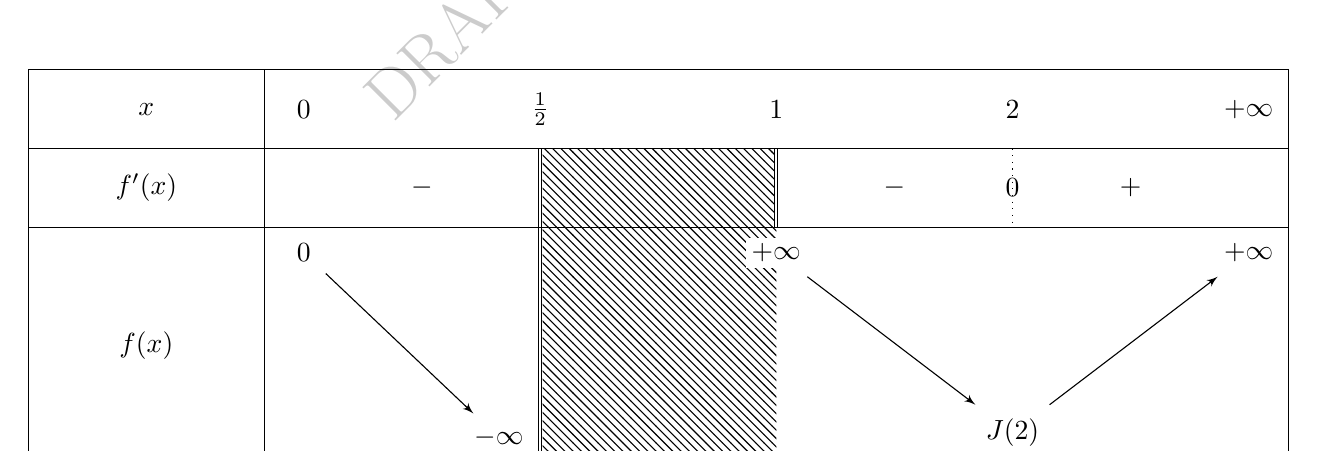
\begin{tikzpicture} 
\tkzTabInit[lgt=3, espcl=3]{$x$ /1, $f'(x)$ /1, $f(x)$ /3}{$0$, $\frac{1}{2}$, $1$, $2$,  $+\infty$} 
\tkzTabLine{, -,d, h, d, -,z ,+,} 
\tkzTabVar{+/$0$, -DH/ $-\infty$, +/$+\infty$ , -/$J(2)$, +/$+\infty$}
\end{tikzpicture} 
\end{center}







\medskip\textbf{Exercice 3}

1) Comparons les intégrales $A$ et $B$ :

$A=\int_{0}^{\frac{\pi}{4}}Ln(\cos x)dx$

$B= \int_{0}^{\frac{\pi}{4}}Ln(\cos(\frac{\pi}{4}- x))dx$.

 En faisant dans $B$ le changement de variable $u =\frac{\pi}{4}- x$, on obtient directement $A = B$.

2. Calculons l'intégrale $I=\int_{0}^{\frac{\pi}{4}}Ln(1+\tan x)dx$.

 On sait que :
 
\[\cos(\frac{\pi}{4}-x)=\frac{\cos x+\sin x}{\sqrt{2}}\]

\[
1+\tan x=\frac{\cos x+\sin x}{\cos x}\]

\begin{align*}
\ln(1+\tan x)&=\ln(\cos x+\sin x)-\ln(\cos x)\\
&=\ln(\sqrt{2})\cos(\frac{\pi}{4}-x)-\ln(\cos x)\\
&=\ln(\sqrt{2})+\ln(\cos(\frac{\pi}{4})-x)-\ln(\cos x)
\end{align*}


D'où, en passant à l'intégrale et comme $A = B$, on a 
\[I=\frac{\pi}{4}\ln(\sqrt{2})\]
 

\end{spacing}
\end{document}
